\chapter{Design}
In this chapter we will explain the applications we developed for this work at a high level. We will skip the experiment automation and plot generation parts of the software, since they are either scripts with a couple of loops that run all the configurations we deemed necessary or simply read data from text files and plot them. Instead, we will be focusing on the two ray tracers we built for this work.

\section{Vulkan Ray Tracer}
\subsection{Rasterized}
The rasterized version of the renderer is quite simple in its design, with a single monolithic Application class handling almost everything and a few helper data structures (Vertex, QueueFamilyIndex, SwapchainSupportDetails and UniformBufferObject) for storing and grouping together information. We see an UML class diagram of this application in figure \ref{rasterized-uml}. This instance of the renderer is much bigger than the following ones due to us not relying on almost any external library and having to handle all the low level operations ourselves, thus resulting in a high ammount of initialization functionality. To all this we added one more class that encapsulates all the performance measuring functionality, which we called FramePerformanceCounter.

\begin{figure}[hbt!]
  \centering
  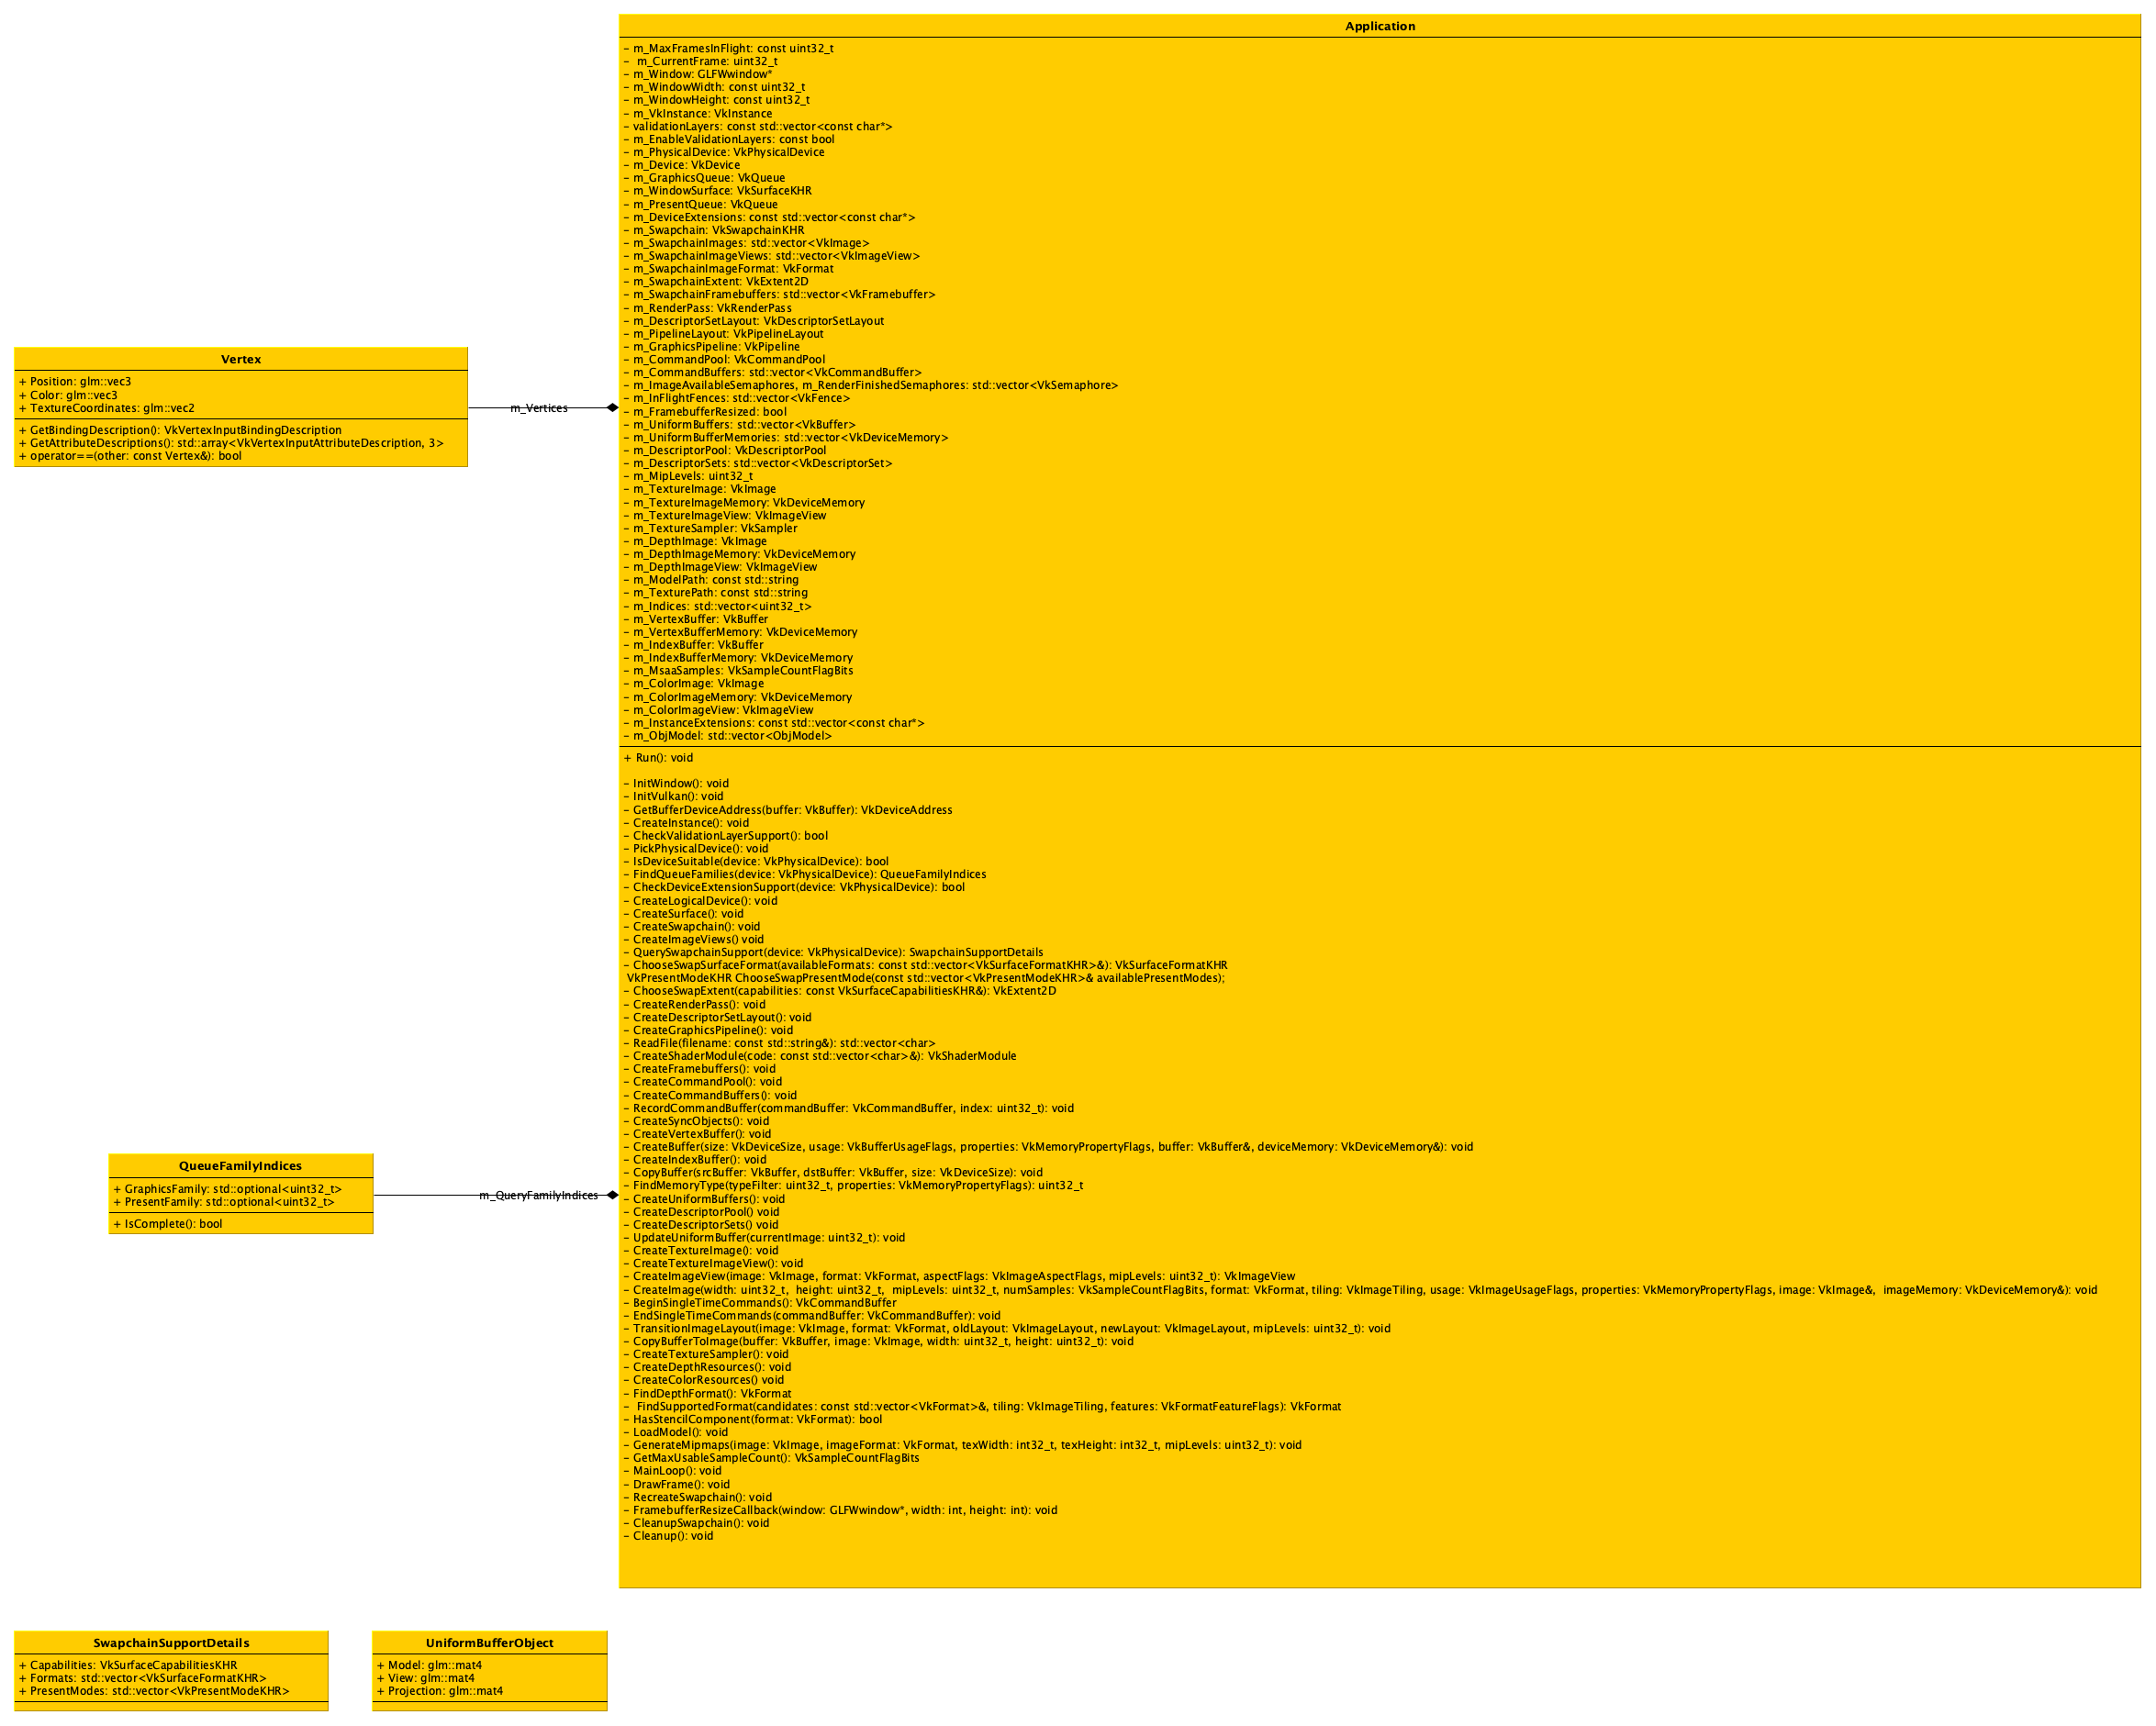
\includegraphics[width=\textwidth]{figuras/rasterized-uml.png}
  \caption{UML class diagram for the rasterized Vulkan renderer.}
  \label{rasterized-uml}
\end{figure}

\subsection{Ray Traced}
For the ray traced version of the Vulkan renderer we refactored and simplified most of the Application class To achieve this, we left an important part of both the initialization and memory cleanup to the Nvvk library. The UML class diagram in figure \ref{vulkan-rt-uml} shows the resulting hierarchy. Finally, we included our own FramePerformanceCounter class for measuring performance.

\begin{figure}[hbt!]
  \centering
  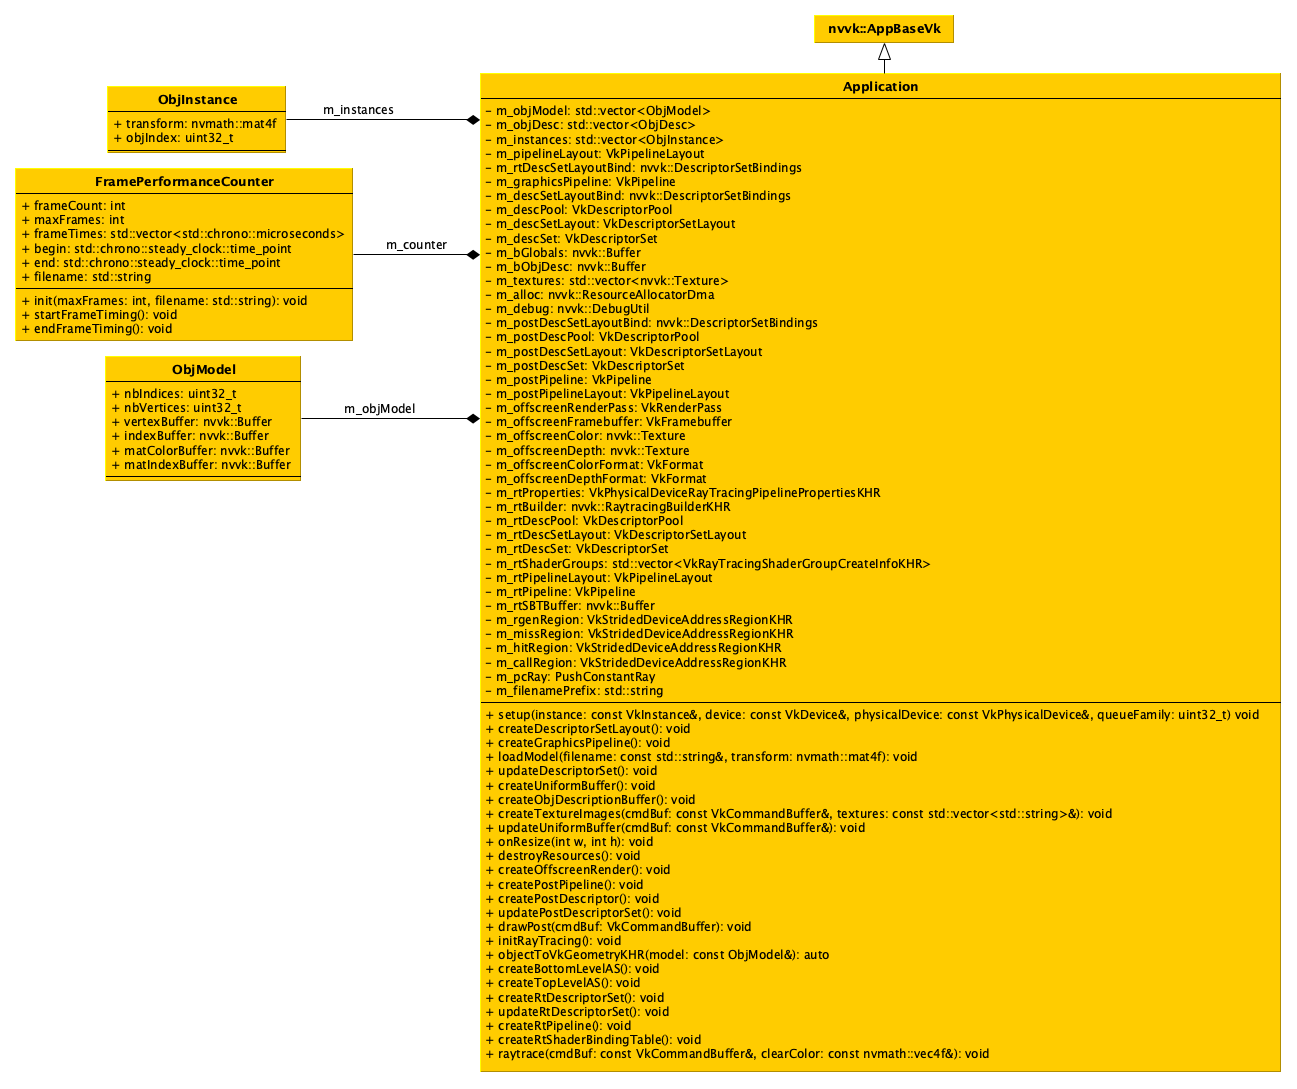
\includegraphics[width=\textwidth]{figuras/vulkan-rt-uml.png}
  \caption{UML class diagram for the raytraced Vulkan renderer.}
  \label{vulkan-rt-uml}
\end{figure}

\clearpage
\section{OptiX Ray Tracer}
For this ray tracer we further encapsulated different functionalities to improve code reusability. This meant increasing the complexity of the class hierarchy. The full diagram can be seen in figure \ref{optix-uml}. 

Here we see a central Renderer class thaat serves much as the Application class from the Vulkan renderer. However, we have encapsulated the window functionality in it's own class hierarchy (GLFWWindow, GLFWCameraWindow). Also, we took the camera manipulation system from the 2019 SIGGRAPH OptiX course \cite{OptixCourse}. This system is highly customizable and perfectly functional, though it adds a fair ammount of complexity to the diagram. This last part includes the classes CameraFrame, CameraFrameManip and it's inheritants. To the class GLFWWindow we also added our FramePerformanceCounter.

\begin{figure}[hbt!]
  \centering
  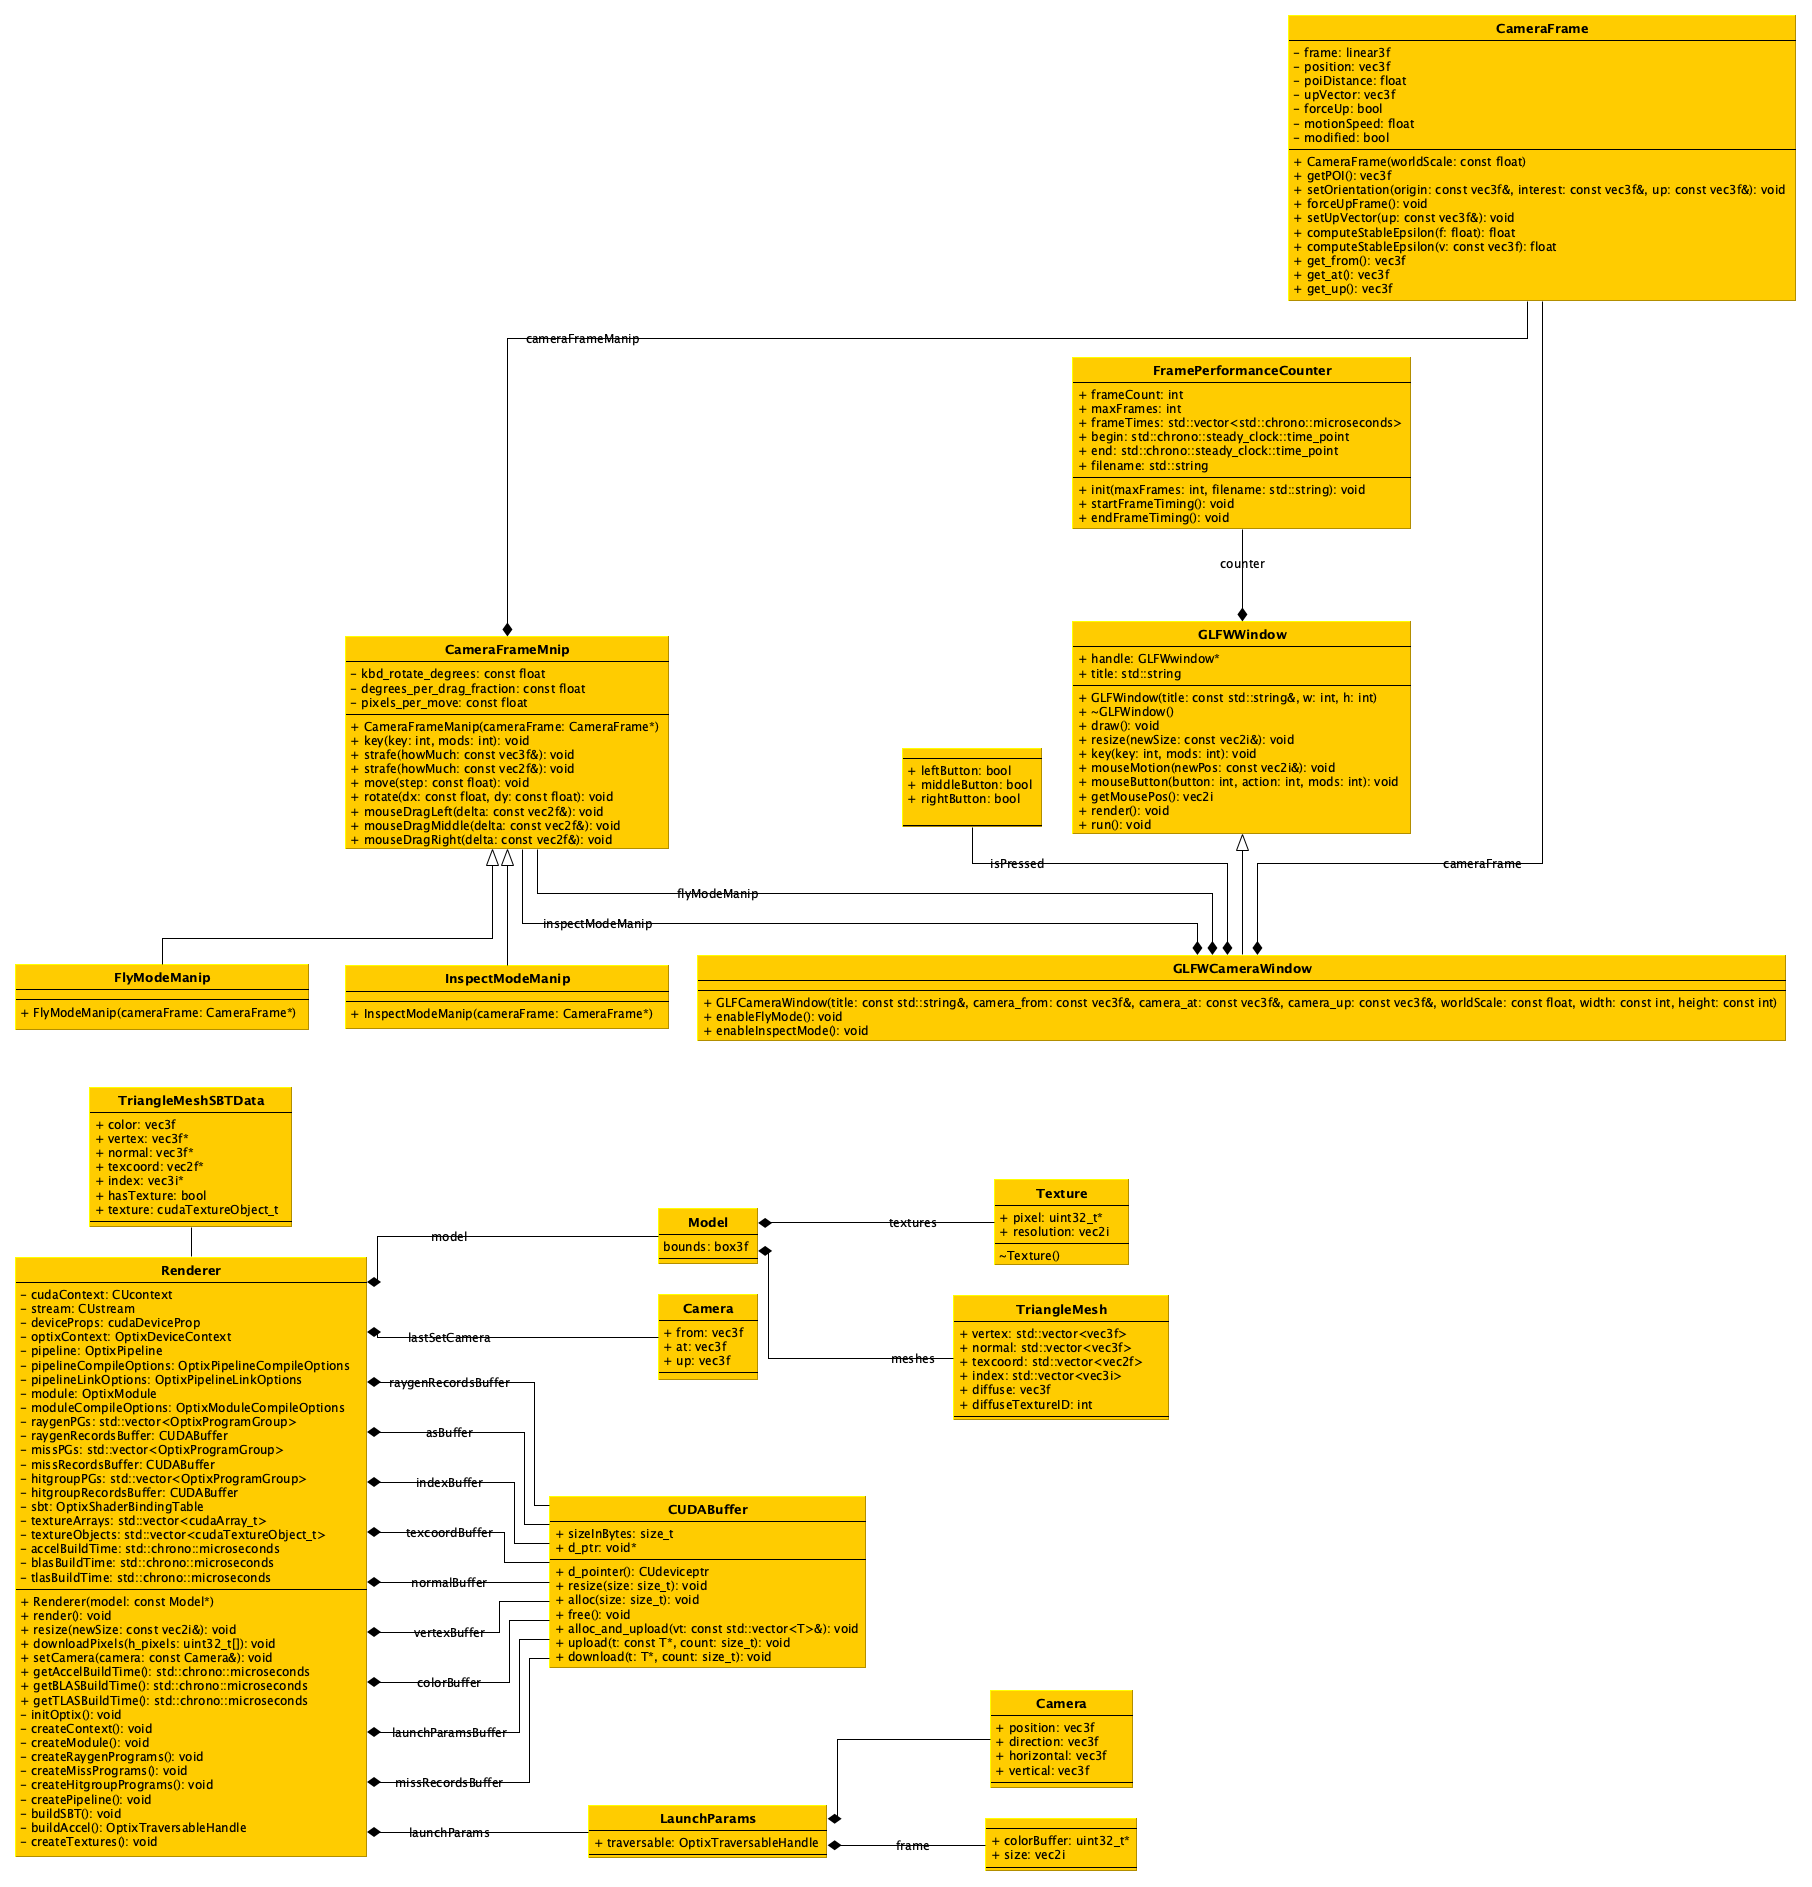
\includegraphics[width=\textwidth]{figuras/optix-uml.png}
  \caption{UML class diagram for the OptiX ray tracer.}
  \label{optix-uml}
\end{figure}

\clearpage
\section{Flow charts}
All the renderers follow the same high level flow. In this section we will be looking at the different processes that they perform. 

\subsection{Initialization}
All renderers start by an initialization process, which we see in detail in figure \ref{init-flowchart}. In this they: 
\begin{enumerate}
\item Read desired window width and height, and model path desired to render, from command line arguments. A couple of fail-safes were placed to have default values for these parameters, in case none were provided. These were added to ease the development process, allowing us to run our software from the development enviroment. 
\item Initialize the windowing and input systems are initialized. Despite some low-level differences these all depend on GLFW, so the process is exactly the same for all renderers.
\item Initialize the renderer itself. This process is highly dependent on each API, but it's mostly sequential, checking the hardware we are running it in is supported and filling data structures. This is specified in detail in the Development chapter.
\item (Only in ray traced renderers) store Acceleration Structure build time, since this process was performed during the renderer initialization.
\item Finally, we get to the main loop, which we'll explain in detail next. After exiting this loop, the program ends.
\end{enumerate}

\begin{figure}[hbt!]
  \centering
  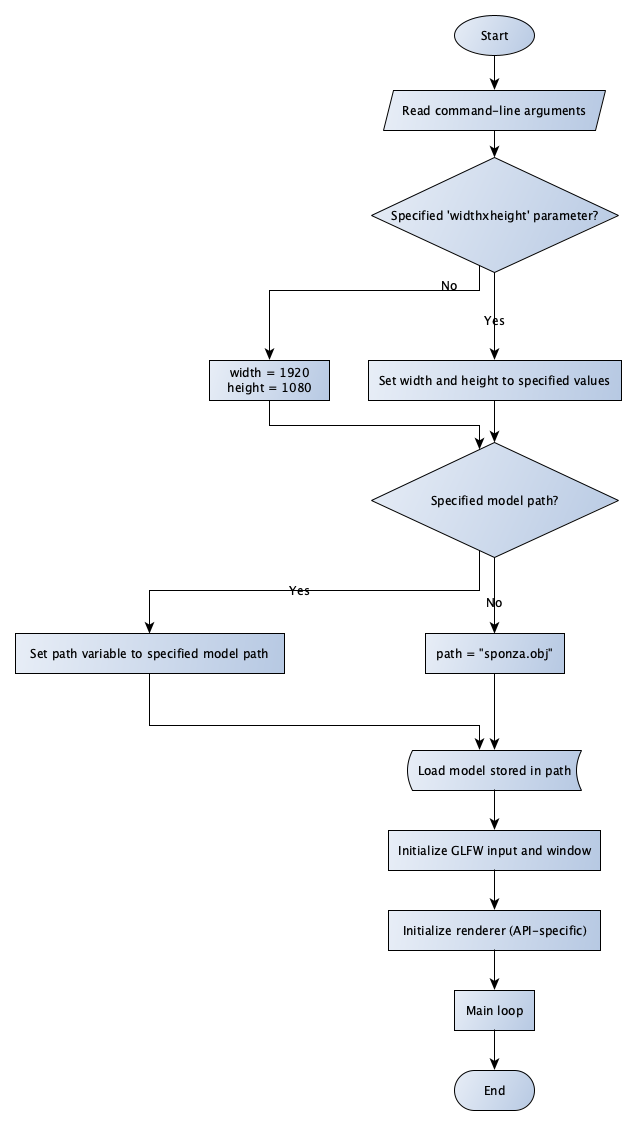
\includegraphics[width=0.75\textwidth]{figuras/init-flowchart.png}
  \caption{Renderer initialization process flow chart.}
  \label{init-flowchart}
\end{figure}

\subsection{Main loop}
Once the renderer is initialized we get to the main loop. This can be seen in figure \ref{main-loop-flowchart}. Ours is not much different than a typical real time graphics applications, with only a couple of additions. Our loop consists mainly on the following steps:

\begin{enumerate}
  \item Initialize our Frame Performance Counter object, in order to store the time taken to render several frames. This process also sets a frame counter to 0.
  \item Check if the operating system is asking to close the window. This is done typically by pressint the "X" button, Alt + F4 or something similar. Most graphics applications mainly depend on this method for deciding when to shut down, however for our automation purposes this wasn't enough, since it would leave the renderer running indefinitely. If the OS has asked to close the window, we jump to step 10. If not, continue to the next step.
  \item Take current time before starting the rendering process.
  \item Render frame to framebuffer. This is done differently in each API, but can be easily isolated from the presentation stage.
  \item Take current time to measure how long it took to render a frame.
  \item Calculate rendering time and store it.
  \item Present rendered frame to screen. This process is separated from the rendering part, so we can know exactly how much it took to simply generate the image. Even though this part is not being measured, we decided to leave it in to monitor what the renderer was doing. In the OptiX ray tracer this is done by displaying the frame buffer's contents as a texture with two triangles that perfectly fit the screen. In the Vulkan ones this is done via the presentation queue.
  \item Increased the rendered frame counter.
  \item Check if the rendered frame counter has reached the limit we set for it, in this case 1000. If it did, continue on. If not, go back to step 2. This is the way in which we automated our tests, automatically finishing the program when reaching a desired limit.
  \item Free any resources left by the renderer. This process varies depending on the API used, but both OptiX (CUDA) and Vulkan require a manual cleanup by the programmer. After this, we end.
\end{enumerate}

In summary, our main loop is mostly the same with a couple of key differences:
\begin{itemize}
  \item[*]{An additional check to terminate the application if we reach a limit (usually 1000) of timed frames.}
  \item[*]{Two separated routines for rendering a frame to a frame buffer and to present this frame buffer to the screen.}
\end{itemize}

\begin{figure}[hbt!]
  \centering
  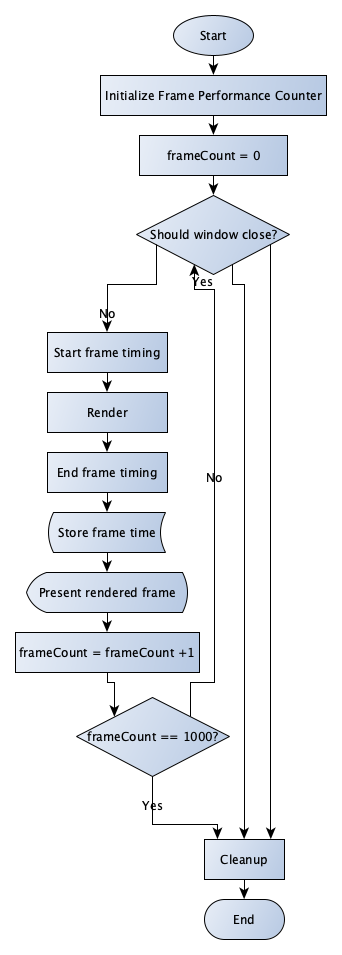
\includegraphics[width=0.5\textwidth]{figuras/main-loop-flowchart.png}
  \caption{Renderer main loop flow chart.}
  \label{main-loop-flowchart}
\end{figure}
